\subsubsection{User-authentication}

\begin{center}
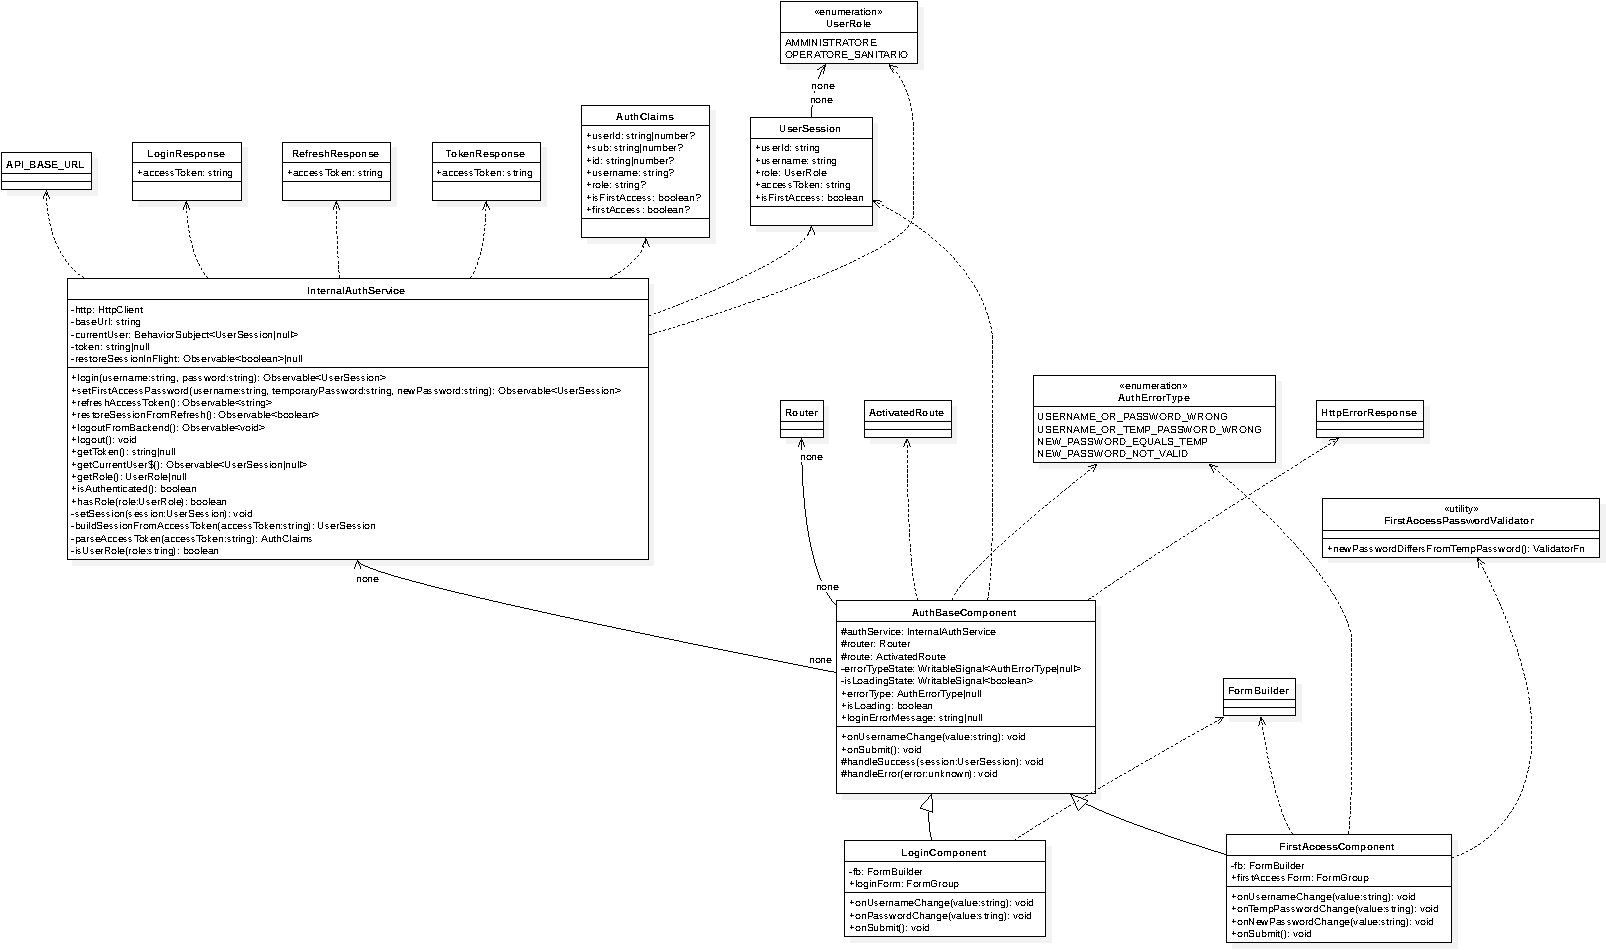
\includegraphics[width=\textwidth]{./frontend/user-auth/user-auth.pdf}
\captionof{figure}{\href{https://snakebyteteam.github.io/3-PB/Documenti_esterni/Specifica_tecnica/frontend/user-auth/user-auth.pdf}{Diagramma delle classi del modulo User authentication}}
\end{center}


\addAtr{\#}{authService: InternalAuthService}{}
\addAtr{\#}{router: Router}{}
\addAtr{\#}{route: ActivatedRoute $|$ null}{}
\addAtr{-}{errorTypeState: WritableSignal$<$AuthErrorType $|$ null$>$}{}
\addAtr{-}{isLoadingState: WritableSignal$<$boolean$>$}{}
\addMet{+}{errorType() : AuthErrorType $|$ null}{Getter che restituisce il tipo di errore corrente leggendo il segnale interno.}
\addMet{+}{errorType(value: AuthErrorType $|$ null) : void}{Setter che aggiorna il tipo di errore corrente nel segnale interno.}
\addMet{+}{isLoading() : boolean}{Getter che restituisce lo stato di caricamento corrente leggendo il segnale interno.}
\addMet{+}{isLoading(value: boolean) : void}{Setter che aggiorna lo stato di caricamento nel segnale interno.}
\addMet{+}{loginErrorMessage() : string $|$ null}{Getter che restituisce il messaggio di errore localizzato corrispondente al tipo di errore corrente.}
\addMet{+}{\textit{onUsernameChange(value: string) : void}}{Metodo astratto che gestisce il cambiamento del valore del campo username.}
\addMet{+}{\textit{onSubmit() : void}}{Metodo astratto che gestisce il submit del form di autenticazione.}
\addMet{\#}{handleSuccess(session: UserSession) : void}{Gestisce il successo dell'autenticazione navigando verso la dashboard o l'URL di ritorno, con supporto al primo accesso.}
\addMet{\#}{handleError(error: unknown) : void}{Gestisce gli errori di autenticazione mappando i codici HTTP nei corrispondenti tipi di errore.}
\makeAbCl{AuthBaseComponent}{Classe astratta base per i componenti di autenticazione, che gestisce lo stato di caricamento, il tipo di errore e la navigazione post-login tramite segnali reattivi. Definisce il contratto per i metodi di submit e cambio username che le sottoclassi devono implementare.}

\addAtr{-}{fb: FormBuilder}{}
\addAtr{+}{firstAccessForm: FormGroup}{}
\addMet{+}{onUsernameChange(value: string) : void}{Aggiorna il valore del campo username nel form di primo accesso.}
\addMet{+}{onTempPasswordChange(value: string) : void}{Aggiorna il valore del campo password temporanea nel form di primo accesso.}
\addMet{+}{onNewPasswordChange(value: string) : void}{Aggiorna il valore del campo nuova password nel form di primo accesso.}
\addMet{+}{onSubmit() : void}{Valida il form e avvia la procedura di impostazione della nuova password, gestendo il successo e l'errore di autenticazione.}
\makeCl{FirstAccessComponent}{Componente Angular per la gestione del primo accesso, che consente all'utente di sostituire la password temporanea con una nuova. Estende AuthBaseComponent e aggiunge la validazione che la nuova password sia diversa da quella temporanea.}

\addAtr{-}{fb: FormBuilder}{}
\addAtr{+}{loginForm: FormGroup}{}
\addMet{+}{onUsernameChange(value: string) : void}{Aggiorna il valore del campo username nel form di login.}
\addMet{+}{onPasswordChange(value: string) : void}{Aggiorna il valore del campo password nel form di login.}
\addMet{+}{onSubmit() : void}{Valida il form e avvia la procedura di autenticazione, gestendo il successo e gli errori tramite i metodi ereditati da AuthBaseComponent.}
\makeCl{LoginComponent}{Componente Angular per la gestione del login, che consente all'utente di autenticarsi tramite username e password. Estende AuthBaseComponent delegando la navigazione post-login e la gestione degli errori alla classe base.}

\addAtr{+}{userId: string}{}
\addAtr{+}{username: string}{}
\addAtr{+}{role: UserRole}{}
\addAtr{+}{accessToken: string}{}
\addAtr{+}{isFirstAccess: boolean}{}
\makeAbCl{UserSession}{Interfaccia che rappresenta la sessione di un utente autenticato. Raccoglie le informazioni identificative, il ruolo, il token di accesso e il flag di primo accesso.}

\addAtr{+}{accessToken: string}{}
\makeAbCl{LoginResponse}{Interfaccia che rappresenta la risposta del backend alla richiesta di login. Espone il token di accesso JWT da utilizzare per le richieste autenticate.}

\addAtr{+}{accessToken: string}{}
\makeAbCl{RefreshResponse}{Interfaccia che rappresenta la risposta del backend alla richiesta di refresh del token. Espone il nuovo token di accesso JWT.}

\addAtr{+}{userId?: string $|$ number}{}
\addAtr{+}{sub?: string $|$ number}{}
\addAtr{+}{id?: string $|$ number}{}
\addAtr{+}{username?: string}{}
\addAtr{+}{role?: string}{}
\addAtr{+}{isFirstAccess?: boolean}{}
\addAtr{+}{firstAccess?: boolean}{}
\makeAbCl{AuthClaims}{Interfaccia che rappresenta i claims estratti dal payload di un token JWT di autenticazione. Gestisce le varianti di nomenclatura dei campi identificativi e del flag di primo accesso.}

\addAtr{+}{accessToken: string}{}
\makeAbCl{TokenResponse}{Interfaccia generica che rappresenta una risposta del backend contenente un token di accesso JWT.}

\addAtr{-}{http: HttpClient}{}
\addAtr{-}{baseUrl: string}{}
\addAtr{-}{currentUser\$: BehaviorSubject$<$UserSession $|$ null$>$}{}
\addAtr{-}{token: string $|$ null}{}
\addAtr{-}{restoreSessionInFlight\$: Observable$<$boolean$>$ $|$ null}{}
\addMet{+}{login(username: string, password: string) : Observable$<$UserSession$>$}{Effettua il login inviando le credenziali al backend e costruisce la sessione utente a partire dal token di accesso ricevuto.}
\addMet{+}{setFirstAccessPassword(username: string, temporaryPassword: string, \\ newPassword: string) : Observable$<$UserSession$>$}{Invia la richiesta di impostazione della nuova password al primo accesso e costruisce la sessione utente dal token ricevuto.}
\addMet{+}{refreshAccessToken() : Observable$<$string$>$}{Rinnova il token di accesso tramite il cookie di refresh e aggiorna la sessione corrente.}
\addMet{+}{restoreSessionFromRefresh() : Observable$<$boolean$>$}{Tenta di ripristinare la sessione utente tramite refresh token, condividendo la richiesta in volo per evitare chiamate concorrenti.}
\addMet{+}{logoutFromBackend() : Observable$<$void$>$}{Invia la richiesta di logout al backend e cancella la sessione locale indipendentemente dall'esito.}
\addMet{+}{logout() : void}{Cancella il token e la sessione utente corrente dallo stato locale.}
\addMet{+}{getToken() : string $|$ null}{Restituisce il token di accesso corrente.}
\addMet{+}{getCurrentUser\$() : Observable$<$UserSession $|$ null$>$}{Restituisce lo stream reattivo della sessione utente corrente.}
\addMet{+}{getRole() : UserRole $|$ null}{Restituisce il ruolo dell'utente corrente, o null se non autenticato.}
\addMet{+}{isAuthenticated() : boolean}{Verifica se l'utente è autenticato controllando la presenza del token e della sessione.}
\addMet{+}{hasRole(role: UserRole) : boolean}{Verifica se il ruolo dell'utente corrente corrisponde a quello specificato.}
\addMet{-}{setSession(session: UserSession) : void}{Aggiorna il token e il BehaviorSubject della sessione con i dati della nuova sessione.}
\addMet{-}{buildSessionFromAccessToken(accessToken: string) : UserSession}{Costruisce l'oggetto sessione estraendo e validando i claims dal payload del token JWT.}
\addMet{-}{parseAccessToken(accessToken: string) : AuthClaims}{Decodifica il payload Base64 del token JWT e lo deserializza nei claims di autenticazione.}
\addMet{-}{isUserRole(role: string) : role is UserRole}{Verifica se la stringa fornita corrisponde a un ruolo utente valido dell'enumerato UserRole.}
\makeCl{InternalAuthService}{Servizio Angular per la gestione dell'autenticazione, che coordina login, logout, refresh del token e ripristino della sessione. Mantiene la sessione utente corrente tramite un BehaviorSubject e gestisce la decodifica e la validazione dei token JWT.}